\section{położenie ogólne}
\begin{defi}
    Powiemy, że punkty $p_1, p_2, \ldots , p_k \in \mathbb{R}^m$ są w \emph{położeniu ogólnym}, jeżeli dla każdego ciągu $l+1$ liczb naturalnych $0< i_0<i_1<\cdots<i_l<k$, $l<m$, punkty $p_{i_0}, p_{i_1},\ldots, p_{i_l}$ tworzą układ afinicznie niezależny.
\end{defi}
\begin{przy}
    Zauważmy, że na płaszczyźnie $\mathbb{R}^2$, zbiór punktów z których każde dowolnie wybrane 3 nie są współliniowe będzie w położeniu ogólnym.
    \begin{figure}[H]
        \centering
        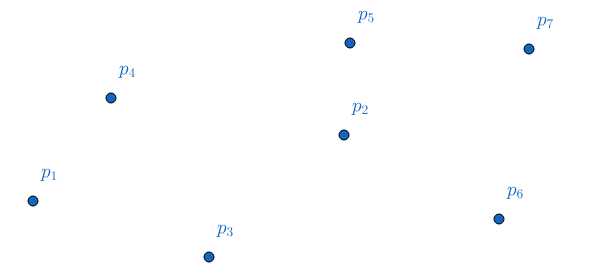
\includegraphics[width=0.5\textwidth]{pictures/polozenie_ogolne.png}
        \caption{Układ w położeniu ogólnym}
        \label{fig:polozenie_ogolne}
    \end{figure}
    Na rysunku \ref{fig:polozenie_ogolne} punkty $p_1, \ldots, p_7$ twożą oczywiście taki układ.
\end{przy}

\begin{twie}
    \label{twie:1_10_2}
    Dla ciągu punktów $q_1, q_2, \ldots, q_k\in \mathbb{R}^m$ i dla każdej liczby $\alpha>0$ istnieją punkty $p_1, p_2, \ldots , p_k\in \mathbb{R}^m$ w położeniu ogólnym, spełniające $\rho (p_i, q_i)<\alpha$$ \forall i=1,2,\ldots,k$.\\
    Ponadto, jeżeli układ $r_1, r_2, \ldots , r_l\in R^m$ jest w położeniu ogólnym, to możemy tak wybrać punkty $p_1, p_2, \ldots , p_k\in R^m$ 
    by $r_1, r_2, \ldots , r_l, p_1, p_2, \ldots , p_k$ również tworzyły układ w położeniu ogólnym.
\end{twie}
\begin{proof}
    Wynika wprost z indukcji:\\
    $p_1$ zdefiniujemy po prostu jako $q_1$, teraz pokażemy krok indukcjyjny.
    Załóżmy że punkty $p_1, \ldots, p_{j-1}$ są dobrze zdefiniowane, czyli tworzą układ w położeniu ogólnym oraz spełniają $\rho(p_i, q_i)<\alpha$ dla $i=1, \ldots, j-1$.\\
    Zauważmy teraz, że każdy co najwyżej $m-1$ elementowy podzbiór punktów $p_1, \ldots, p_{j-1}$ jest afinicznie niezależny, oraz że będą one rozpinały przestrzeń afiniczną wymiaru co najwyżej $m-1$. Czyli jest to zbiór nigdzie gęsty w $\mathbb{R}^m$. Ponieważ wszystkich takich podzbiorów jest skończenie wiele, to suma przestrzeni afinicznych rozpiętych na nich również będzie nigdzie gęsta. Wynika z tego, jesteśmy w stanie znaleźć taki punkt $p_j$ poza tym zbiorem, który będzie spełniał $\rho (p_j, q_j)<\alpha$.\\
    \\
    Dowód dla drugiej części twierdzenia jest analogiczny. 
    \begin{figure}[H]
        \centering
        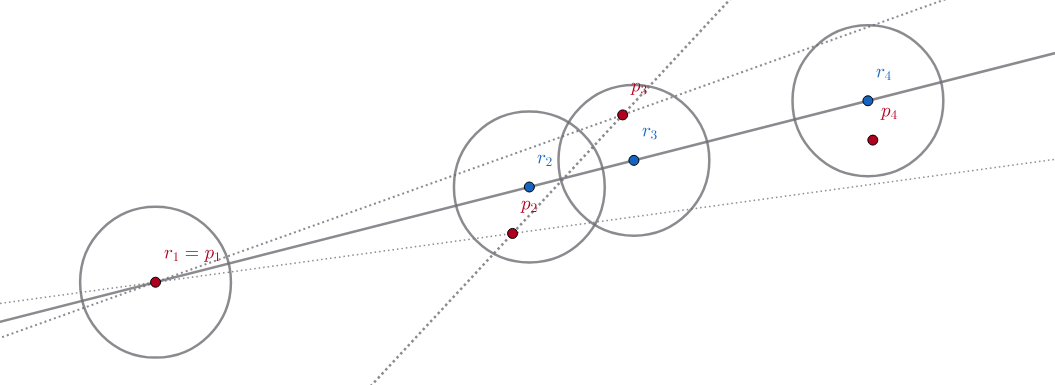
\includegraphics[width=0.8\textwidth]{pictures/polo_tw_konstrukcja.png}
        \caption{Szkic konstrukcji}
        \label{fig:szkic}
    \end{figure}
\end{proof}


\section{Nerw}

\begin{defi}
    \cite{alex1927} 
    Niech $\mathcal{U} = \{U_i\}_{i=1}^k$ będzie skończonym otwartym pokryciem przestrzeni topologicznej $X$.
    \emph{Nerwem} pokrycia $\mathcal{U}$ nazwiemy dowolny kompleks symplicjalny $\mathcal{N(U)}$, 
    którego wierzchołki możemy ustawić w ciąg $p_1, p_2, \ldots, p_k$ w taki sposób, że
    \[p_{i_0}p_{i_1} \ldots p_{i_m}\in \mathcal{N(U)} \Leftrightarrow U_{i_0}\cap U_{i_1}\cap \cdots \cap U_{i_m}\neq \emptyset \]
\end{defi}
\begin{przy}
    \begin{figure}[H]
        \centering
        % 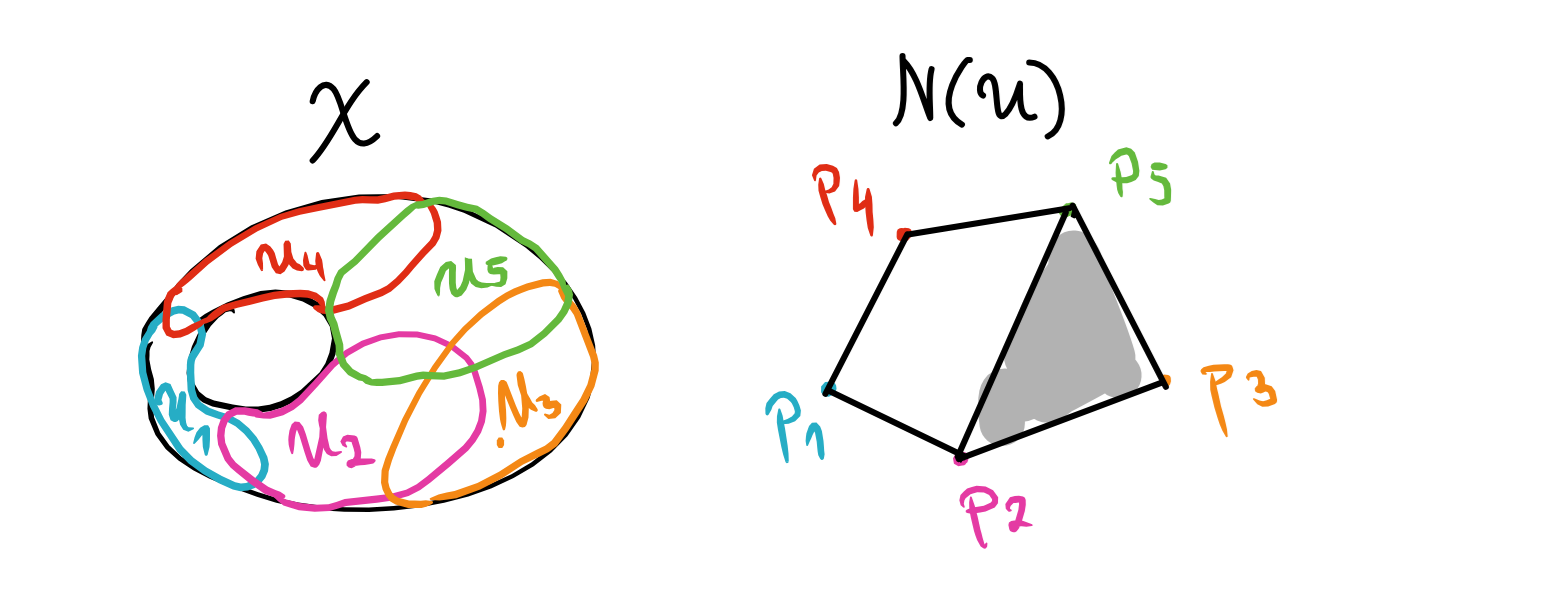
\includegraphics[width=0.8\textwidth]{pictures/nerw_2.png}
        \resizebox{0.7\textwidth}{!}{%
\definecolor{colCyan}{RGB}{0, 168, 204}
\definecolor{colRed}{RGB}{220, 50, 32}
\definecolor{colGreen}{RGB}{92, 172, 45}
\definecolor{colPink}{RGB}{225, 60, 140}
\definecolor{colOrange}{RGB}{245, 130, 32}
\definecolor{colGray}{RGB}{180, 180, 180}

\centering

\begin{tikzpicture}[line cap=round, line join=round]

% ================= Lewy diagram: Przestrzeń X (zmniejszony) =================
\begin{scope}[local bounding box=left, scale=0.45]
  % Tytuł
  \node at (3.5, 7) {\Huge $\mathcal{X}$};

  % Współrzędne P
  {
  \coordinate (P1) at (-4, 0);
  \coordinate (P2) at (-3.1, 2);
  \coordinate (P3) at (-2, 3);
  \coordinate (P4) at (0.0, 3.8);
  \coordinate (P5) at (2, 4.2);
  \coordinate (P6) at (3.5, 4.3);
  \coordinate (P7) at (5.3, 4.2);
  \coordinate (P8) at (7, 4);
  \coordinate (P9) at (9, 3);
  \coordinate (P10) at (10, 1);
  \coordinate (P11) at (10.1, -0.6);
  \coordinate (P12) at (10, -2);
  \coordinate (P13) at (9.5, -3.2);
  \coordinate (P14) at (8.7, -4.4);
  \coordinate (P15) at (7,-5);
  \coordinate (P16) at (5, -5.3);
  \coordinate (P17) at (3, -5.3);
  \coordinate (P18) at (1, -5);
  \coordinate (P19) at (-0.7, -4.4);
  \coordinate (P20) at (-2, -3.8);
  \coordinate (P21) at (-3, -3);
  \coordinate (P22) at (-3.8, -1.6);
  \coordinate (P23) at (-3.6, 1.2);

  % Współrzędne R
  \coordinate (R1) at (-0.8, 0);
  \coordinate (R2) at (-0.2, 1.4);
  \coordinate (R3) at (1, 2);
  \coordinate (R4) at (2,2.1);
  \coordinate (R5) at (2.8, 1.9);
  \coordinate (R6) at (3.5,1.5);
  \coordinate (R7) at (4,1);
  \coordinate (R8) at (4.2,0.3);
  \coordinate (R9) at (4,-0.6);
  \coordinate (R10) at (3,-1.6);
  \coordinate (R11) at (1.7, -1.8);
  \coordinate (R12) at (0.5,-1.5);
  \coordinate (R13) at (-0.4, -0.8);
  \coordinate (R14) at (-0.7, 0.8);

  % Współrzędne U
  \coordinate (U1) at (-1.2, 2.9);
  \coordinate (U2) at (-1.6, 1);
  \coordinate (U3) at (-0.8, -1.8);
  \coordinate (U4) at (1.6, -3.8);
  \coordinate (U5) at (5.2, -0.4);
  \coordinate (U6) at (3.6, 2.6);
  \coordinate (U7) at (6.4, 3.6);
  \coordinate (U8) at (4.8, 1.5);
  \coordinate (U9) at (1,-2);
  \coordinate (U10) at (0, -4.4);
  \coordinate (U11) at (-0.1, 2.1);
  \coordinate (U12) at (-2.6, 2.4);
  \coordinate (U13) at (-2.7, 1);
  \coordinate (U14) at (-1.2, -3);
  \coordinate (U15) at (7.6, -3.4);
  \coordinate (U16) at (4.2, -1.4);
  \coordinate (U17) at (9.1, -1.4);
  \coordinate (U18) at (4.2, 3.7);
  \coordinate (U19) at (5.1, -3.8);
  \coordinate (U20) at (7.8, 1);
  \coordinate (U21) at (7.6, -0.7);

  % Rysowanie punktów P, R, U
  % \foreach \p in {P1,...,P23} \fill[black!100] (\p) circle (3pt);
  % \foreach \p in {R1,...,R14} \fill[black!100] (\p) circle (3pt);
  % \foreach \p in {U1,...,U21} \fill[black!100] (\p) circle (3pt);

  % % Etykiety P
  % \foreach \i in {1,...,23} \node[colRed, above left=2pt] at (P\i) {\Large $P_{\i}$};

  % % Etykiety R
  % \foreach \i in {1,...,14} \node[colGreen, above left=2pt] at (R\i) {\Large $R_{\i}$};

  % % Etykiety U (czarne)
  % \foreach \i in {1,...,21} \node[black!100, above left=2pt] at (U\i) {\Large $U_{\i}$};
  }

  % Zewnętrzna granica
  \draw[line width=5pt, black!100] plot [smooth cycle, tension=0.6] coordinates {
    (P1) (P23) (P2) (P3) (P4) (P5) (P6) (P7) (P8) (P9) 
    (P10) (P11) (P12) (P13) (P14) 
    (P15) (P16) (P17) (P18) (P19) 
    (P20) (P21) (P22) 
  };

  % Wewnętrzna granica R
  \draw[line width=5pt, black!100] plot [smooth cycle, tension=0.6] coordinates {
    (R1) (R14) (R2) (R3) (R4) (R5) 
    (R6) (R7) (R8) (R9)  
    (R10) (R11) (R12) (R13) 
  };

  % Kształty U
  \draw[line width=4pt, colCyan] plot [smooth cycle, tension=0.6] coordinates {
    (P1) (P23) (P2) (U12) 
    (U1) (U11) (R2) (R14) (R1) 
    (R13) (U9) (U4) (U10) (P20) (P21) (P22) 
  };

  \draw[line width=4pt, colRed] plot [smooth cycle, tension=0.6] coordinates {
    (U2) (U13) (P2) (P3) (P4) 
    (P5) (P6) (P7) (U7) 
    (U8) (R6) (R5) 
    (R4) (R3) (R2) 
  };

  \draw[line width=4pt, colPink] plot [smooth cycle, tension=0.6] coordinates {
    (U3) (R12) (R11) (R10) 
    (R9) (U5) (U21) (U15) (P15) 
    (P16) (P17) (P18) (P19) 
    (U14)
  };

  \draw[line width=4pt, colGreen] plot [smooth cycle, tension=0.6] coordinates {
    (R7) (R6) (U6) (U18) (P7) 
    (P8) (P9) (P10) (U17)
    (U16) (R9) (R8) 
  };

  \draw[line width=4pt, colOrange] plot [smooth cycle, tension=0.6] coordinates {
    (U19) (U20) (P10) (P11) 
    (P12) (P13) (P14) 
    (P15) 
  };

  % Duże etykiety U
  \node[colCyan] at (-2,-0.5) { \fontsize{17}{48}\selectfont $U_1$ };
  \node[colPink] at (3.5,-3.2) { \fontsize{17}{48}\selectfont $U_2$ };
  \node[colOrange] at (8.7,-2.5) { \fontsize{17}{48}\selectfont $U_3$ };
  \node[colRed] at (1.7,3.1) { \fontsize{17}{48}\selectfont $U_4$ };
  \node[colGreen] at (6.3,1.2) { \fontsize{17}{48}\selectfont $U_5$ };
\end{scope}

% ================= Prawy diagram: Nerw N(u) (oryginalny rozmiar) =================
\begin{scope}[local bounding box=right, shift={($(left.east)+(2.5cm,-0.2)$)}]
  % Tytuł
  \node at (1.5, 2.7) {\Huge $\mathcal{N(U)}$};

  % Współrzędne wierzchołków
  \coordinate (N1) at (-0.5, -1.3);
  \coordinate (N4) at (1.5, 1.3);
  \coordinate (N5) at (4, 1.7);
  \coordinate (N2) at (2, -2.3);
  \coordinate (N3) at (5.2, -0.6);

  % Zacieniony 2-sympleks
  \fill[colGray] (N2) -- (N5) -- (N3) -- cycle;

  % Krawędzie kompleksu
  \draw[line width=3pt, black] (N1) -- (N4) -- (N5) -- (N3) -- (N2) -- cycle;
  \draw[line width=3pt, black] (N2) -- (N5);

  % Wierzchołki
  \fill[colCyan] (N1) circle (5pt);
  \fill[colRed] (N4) circle (5pt);
  \fill[colGreen] (N5) circle (5pt);
  \fill[colPink] (N2) circle (5pt);
  \fill[colOrange] (N3) circle (5pt);

  % Etykiety wierzchołków
  \node[colCyan, below left=2pt] at (N1) {\fontsize{17}{48}\selectfont $P_1$};
  \node[colRed, above left=2pt] at (N4) {\fontsize{17}{48}\selectfont  $P_4$};
  \node[colGreen, above right=2pt] at (N5) {\fontsize{17}{48}\selectfont $P_5$};
  \node[colPink, below=4pt] at (N2) {\fontsize{17}{48}\selectfont  $P_2$};
  \node[colOrange, right=4pt] at (N3) {\fontsize{17}{48}\selectfont  $P_3$};
\end{scope}

\end{tikzpicture}
}
        \caption{nerw}
        \label{fig:nerw_2}
    \end{figure}
    dodać jakiś opis
\end{przy}
\section{twierdzenie o zanużeniu w $R^{2n+1}$}

\begin{twie}
    Niech $\mathcal{U}=\{U_i\}_{i=1}^k$ będzie skończonym otwartym pokryciem przestrzeni topologicznej $X$. Jeżeli krotność pokrycia $\mathcal{U}$ jest conajwyżej $n$, to nerw pokrycia $\mathcal{N(U)}$ możemy zrealizować w $\mathbb{R}^{2n+1}$. \\
    Ponadto, mając:
    \begin{itemize}
        \item $H$ - n-wymiarową podprzestrzeń afiniczną  $R^{2n+1}$,
        \item punkty $q_1, \ldots, q_k\in R^{2n+1}$,
        \item liczbę $\alpha>0$
    \end{itemize} 
    możemy wybrać nerw $\mathcal{N(U)}$ w taki sposób, by $\mathcal{N(U)}$ nie przecinał podprzestrzeni $H$, oraz by $p_1, \ldots, p_k$ wierzchołki nerwu $\mathcal{N(U)}$ spełniały $\rho(p_i, q_i)<\alpha$ dla $i=1,2,\ldots, k$
\end{twie}
\begin{proof}
    Możemy łatwo zauważyć, że druga część twierdzenia jest rozszerzeniem pierwszej, możemy się więc skupić na udowodnieniu tylko drugiej części.\\
    Niech $r_1, \ldots, r_{n+1}\in R^{2n+1}$ afinicznie niezależne rozpinające $H$.
    Z twierdzenia \ref{twie:1_10_2} wiemy, że możemy tak wybrać punkty $p_1, \ldots, p_k\in \mathbb{R}^{2n+1}$ by punkty $r_1, \ldots, r_{n+1}, p_1,\ldots, p_k $ były w położeniu ogólnym. \\
    Z tego, że $\ord \mathcal{U}\le n$ wiemy, że dla każdego ciągu $l+1$ indeksów $0\le i_0< \cdots < i_l\le k$ takich że $U_{i_0}\cap\cdots \cap U_{i_l}\ne \emptyset$, to $l\le n<2n+1$, czyli punkty odpowiadające tym indeksom: $p_{i_0},\ldots p_{i_l}$ tworzą układ afinicznie niezależny oraz że sympleks na nich zbudowany jest dobrze zdefiniowany. \\
    Teraz niech $\mathcal{K}$ będzie rodziną sympleksów zdefiniowanych w ten sposób. Teraz pozostaje pokazć, że tak zdefiniowana rodzina jest nerwem $\mathcal{N(U)}$ oraz że $\mathcal{N(U)}\cap H=\emptyset$.\\
    Zauważmy, że do pokazania że $\mathcal{K}$ jest nerwem, jedyne co trzeba pokazać to że $\mathcal{K}$ jest kompleksem symplicjalnym, czyli że 
    \begin{enumerate}
        \item dla każdego sympleksu $S\in \mathcal{K}$ każda jego ściana $S'$ również spełnia $S'\in \mathcal{K}$
        \item dla każdych $S_1, S_2\in \mathcal{K}$, jeżeli $S_1\cap S_2\ne \emptyset$ to $S_1\cap S_2$ musi być ścianą obu.
    \end{enumerate}
    dowód 1:\\
    Zauważmy, że skoro sympleks w $S$ oparty na wierzchołkach $p_{i_0}, \ldots, p_{i_l}$ jest w $\mathcal{K}$, to $U_{i_0}\cap\cdots\cap U_{i_l}\ne \emptyset$. Za tym od razu idzie że przecięcie każdego podzbioru $\{ U_{i_0}, \ldots, U_{i_l}\}$ musi również być niepuste, tak więc każda ściana $S$ również będzie należała do $\mathcal{K}$.
    \\
    dowód 2:\\
    Weźmy $S_1, S_2\in \mathcal{K}$, $S_1$ oparty na $p_{i_0}, \ldots, p_{i_l}$, $S_2$ oparty na $p_{j_0}, \ldots, p_{j_m}$, $l, m\le n$.\\
    Załóżmy, że sympleksy oparte są na dokładnie $0\le a\le \min(l+1, m+1)$ takich samych wierzchołkach. Możemy w takim razie tak je przeindeksować, by spełnione było:
    \[p_{i_s}=p_{j_s} \;\; \mathrm{dla} \;\;s=0,1,\ldots, a-1\]
    \[p_{i_a}, \ldots, p_{i_l}, p_{j_a},\ldots,  p_{j_m}\;\; \mathrm{parami\;\;różne}\]
    Weźmy dowolny punkt $p$ należący do przecięcia $S_1\cap S_2$. Zauważmy że skoro $p\in S_1$, to możemy przedstawić punkt $p$ jako:
    \[p=\sum _{s=0}^l \lambda_sp_{i_s}, \;\; \sum_{s=0}^l\lambda_s=1,
    \lambda_s\ge 0\forall_{s=0,1, \ldots, l} \]
    podobnie z $p\in S_2$ dostajemy:
    \[p=\sum _{t=0}^m \lambda'_tp_{i_t}, \;\; \sum_{t=0}^m\lambda'_t=1,
    \lambda'_t\ge 0\forall_{t=0,1, \ldots, m} \]
    Dostajemy w takim razie układ równań:
    \[\sum _{s=0}^l \lambda_sp_{i_s}- \sum _{t=0}^m \lambda'_tp_{i_t} = 
    0\]
    \[\sum _{s=0}^l \lambda_s - \sum _{t=0}^m \lambda'_t = 0\]
    Pierwsze równanie możemy uprościć do postaci:
    \[
    \sum _{s=0}^a (\lambda_s-\lambda'_s)p_{i_s} +
    \sum _{s=a}^l \lambda_sp_{i_s}- \sum _{t=a}^m \lambda'_tp_{i_t} = 
    0\]
    Zauważmy, że skoro $l, m\le n$, czyli $2+m+l\le 2n+2$, to punkty 
    $p_{i_0}, \ldots, p_{i_l},p_{j_a}\ldots ,p_{j_m}$ będą tworzyły układ afinicznie niezależny, z czego wynika że wszystkie wpółczynniki w powyższym równianiu muszą być równe 0, za czym idzie:
    \[\lambda_s=\lambda'_s,  \;\;\mathrm{dla}\;\;s=0,\ldots, a-1 \]
    \[\lambda_s = 0, \;\;\mathrm{dla}\;\;s=a, \ldots,l\]
    \[\lambda'_s=0,  \;\;\mathrm{dla}\;\;\;s=a,\ldots, m\]
    W takim razie punkt $p$ możemy rozpisać jako
    \[p=\sum_{s=0}^{a-1}\lambda_sp_{i_s}=\sum_{s=0}^{a-1}\lambda'_sp_{j_s}\]
    czyli punkt $p$ należy również do sympleksu opartego na $p_{i_0}, \ldots, p_{i_{a-1}}$, który jest ścianą obu sympleksów $S_1, S_2$, co kończy dowód.
    Wynika z tego, że $\mathcal{K}$ faktycznie jest nerwem pokrycia $\mathcal{U}$.\\
    Do skończenia dowodu twierdzenia wystarczy pokazać, że $H\cap \mathcal{K}=\emptyset$, jest to jednak analogiczne do powyższego.
\end{proof}